\documentclass{standalone}
\usepackage{tikz}
\usetikzlibrary{patterns, positioning}

\begin{document}
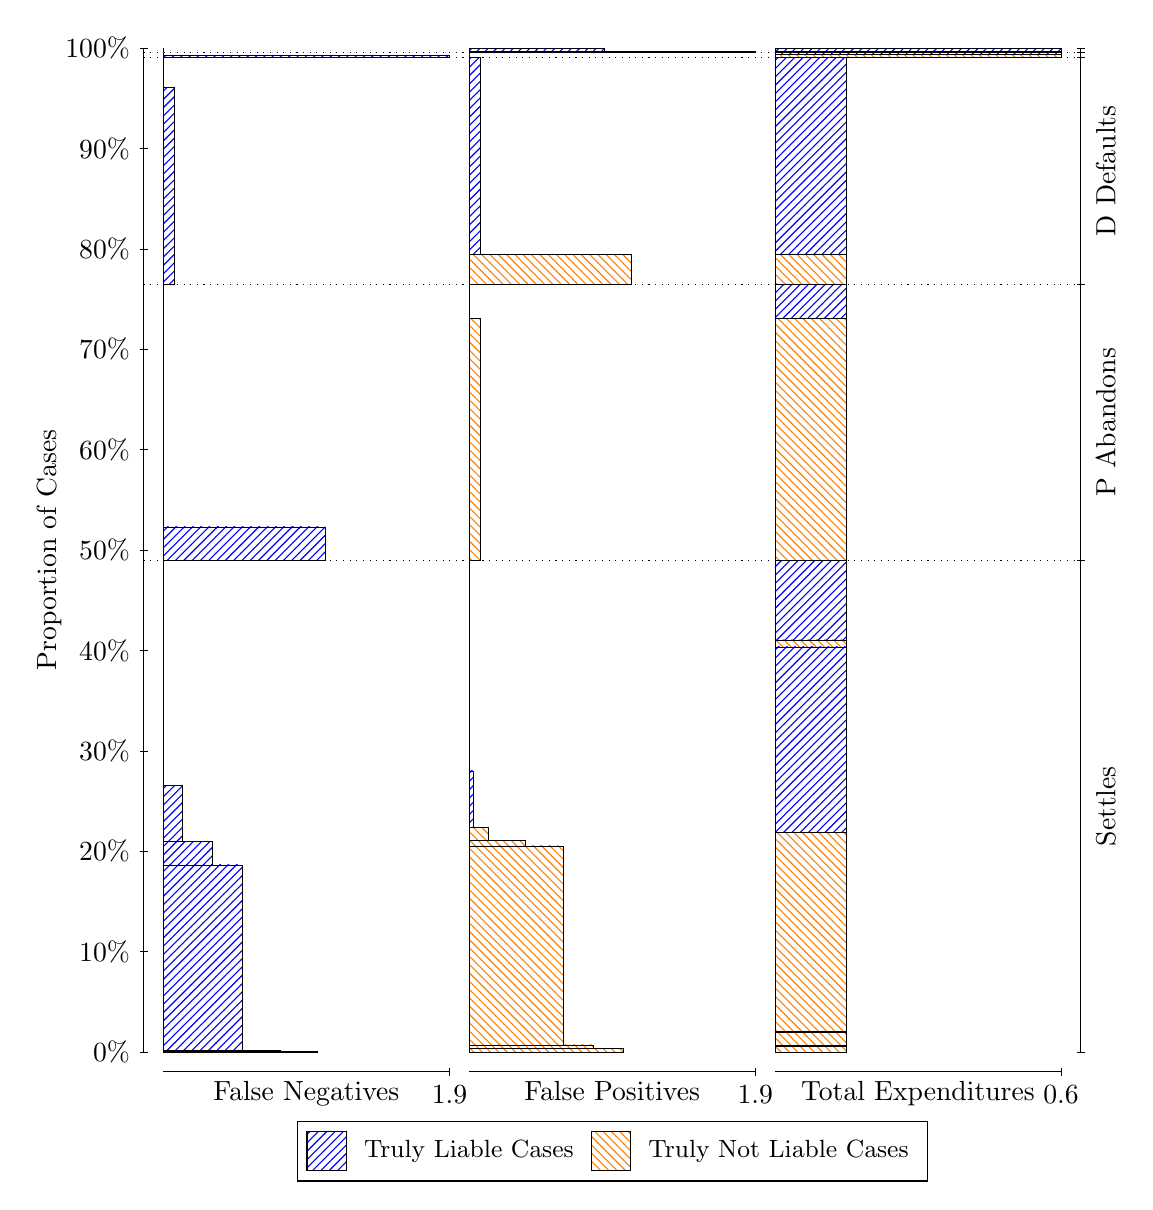
\begin{tikzpicture}
\draw[black, very thin] (1.5,1.75) -- (1.5,14.5);
\node[rotate=90, anchor=center] at (0.3, 8.125) {Proportion of Cases};
\draw[black, very thin] (1.45,1.75) -- (1.55,1.75);
\node[anchor=east] at (1.45, 1.75) {0\%};
\draw[black, very thin] (1.45,3.025) -- (1.55,3.025);
\node[anchor=east] at (1.45, 3.025) {10\%};
\draw[black, very thin] (1.45,4.3) -- (1.55,4.3);
\node[anchor=east] at (1.45, 4.3) {20\%};
\draw[black, very thin] (1.45,5.575) -- (1.55,5.575);
\node[anchor=east] at (1.45, 5.575) {30\%};
\draw[black, very thin] (1.45,6.85) -- (1.55,6.85);
\node[anchor=east] at (1.45, 6.85) {40\%};
\draw[black, very thin] (1.45,8.125) -- (1.55,8.125);
\node[anchor=east] at (1.45, 8.125) {50\%};
\draw[black, very thin] (1.45,9.4) -- (1.55,9.4);
\node[anchor=east] at (1.45, 9.4) {60\%};
\draw[black, very thin] (1.45,10.675) -- (1.55,10.675);
\node[anchor=east] at (1.45, 10.675) {70\%};
\draw[black, very thin] (1.45,11.95) -- (1.55,11.95);
\node[anchor=east] at (1.45, 11.95) {80\%};
\draw[black, very thin] (1.45,13.225) -- (1.55,13.225);
\node[anchor=east] at (1.45, 13.225) {90\%};
\draw[black, very thin] (1.45,14.5) -- (1.55,14.5);
\node[anchor=east] at (1.45, 14.5) {100\%};

\draw[black, very thin] (13.4,1.75) -- (13.4,14.5);
\draw[black, very thin] (13.35,1.75) -- (13.45,1.75);
\node[anchor=west] at (13.35, 1.75) {};
\draw[black, very thin] (13.35,7.9928) -- (13.45,7.9928);
\node[anchor=west] at (13.35, 7.9928) {};
\draw[black, very thin] (13.35,11.496) -- (13.45,11.496);
\node[anchor=west] at (13.35, 11.496) {};
\draw[black, very thin] (13.35,14.383) -- (13.45,14.383);
\node[anchor=west] at (13.35, 14.383) {};
\draw[black, very thin] (13.35,14.441) -- (13.45,14.441);
\node[anchor=west] at (13.35, 14.441) {};
\draw[black, very thin] (13.35,14.5) -- (13.45,14.5);
\node[anchor=west] at (13.35, 14.5) {};

\draw[black, very thin, pattern color=blue, pattern=north east lines] (1.75,1.75) rectangle (3.7101,1.7605);
\draw[black, very thin, pattern color=blue, pattern=north east lines] (1.75,1.7605) rectangle (3.232,1.771);
\draw[black, very thin, pattern color=blue, pattern=north east lines] (1.75,1.771) rectangle (2.8496,1.7712);
\draw[black, very thin, pattern color=blue, pattern=north east lines] (1.75,1.7712) rectangle (2.7539,4.1254);
\draw[black, very thin, pattern color=blue, pattern=north east lines] (1.75,4.1254) rectangle (2.3715,4.4217);
\draw[black, very thin, pattern color=blue, pattern=north east lines] (1.75,4.4217) rectangle (1.989,5.136);
\draw[black, very thin, pattern color=orange, pattern=north west lines] (1.75,5.136) rectangle (1.75,7.9928);
\draw[black, very thin, pattern color=blue, pattern=north east lines] (1.75,7.9928) rectangle (3.8057,8.4188);
\draw[black, very thin, pattern color=orange, pattern=north west lines] (1.75,8.4188) rectangle (1.75,11.496);
\draw[black, very thin, pattern color=blue, pattern=north east lines] (1.75,11.496) rectangle (1.8934,14);
\draw[black, very thin, pattern color=orange, pattern=north west lines] (1.75,14) rectangle (1.75,14.383);
\draw[black, very thin, pattern color=blue, pattern=north east lines] (1.75,14.383) rectangle (5.3833,14.404);
\draw[black, very thin, pattern color=orange, pattern=north west lines] (1.75,14.404) rectangle (1.75,14.441);
\draw[black, very thin, pattern color=orange, pattern=north west lines] (1.75,14.441) rectangle (1.75,14.462);
\draw[black, very thin, pattern color=blue, pattern=north east lines] (1.75,14.462) rectangle (1.75,14.5);
\draw[black, very thin, pattern color=orange, pattern=north west lines] (5.6333,1.75) rectangle (7.5934,1.7938);
\draw[black, very thin, pattern color=orange, pattern=north west lines] (5.6333,1.7938) rectangle (7.211,1.8389);
\draw[black, very thin, pattern color=orange, pattern=north west lines] (5.6333,1.8389) rectangle (6.8285,4.3666);
\draw[black, very thin, pattern color=orange, pattern=north west lines] (5.6333,4.3666) rectangle (6.7329,4.3668);
\draw[black, very thin, pattern color=orange, pattern=north west lines] (5.6333,4.3668) rectangle (6.3504,4.436);
\draw[black, very thin, pattern color=orange, pattern=north west lines] (5.6333,4.436) rectangle (5.8724,4.6068);
\draw[black, very thin, pattern color=blue, pattern=north east lines] (5.6333,4.6068) rectangle (5.6811,5.3211);
\draw[black, very thin, pattern color=blue, pattern=north east lines] (5.6333,5.3211) rectangle (5.6333,7.9928);
\draw[black, very thin, pattern color=orange, pattern=north west lines] (5.6333,7.9928) rectangle (5.7768,11.07);
\draw[black, very thin, pattern color=blue, pattern=north east lines] (5.6333,11.07) rectangle (5.6333,11.496);
\draw[black, very thin, pattern color=orange, pattern=north west lines] (5.6333,11.496) rectangle (7.689,11.879);
\draw[black, very thin, pattern color=blue, pattern=north east lines] (5.6333,11.879) rectangle (5.7768,14.383);
\draw[black, very thin, pattern color=orange, pattern=north west lines] (5.6333,14.383) rectangle (5.6333,14.42);
\draw[black, very thin, pattern color=blue, pattern=north east lines] (5.6333,14.42) rectangle (5.6333,14.441);
\draw[black, very thin, pattern color=orange, pattern=north west lines] (5.6333,14.441) rectangle (9.2667,14.462);
\draw[black, very thin, pattern color=blue, pattern=north east lines] (5.6333,14.462) rectangle (7.3544,14.5);
\draw[black, very thin, pattern color=orange, pattern=north west lines] (9.5167,1.75) rectangle (10.425,1.8192);
\draw[black, very thin, pattern color=blue, pattern=north east lines] (9.5167,1.8192) rectangle (10.425,1.8297);
\draw[black, very thin, pattern color=orange, pattern=north west lines] (9.5167,1.8297) rectangle (10.425,2.0005);
\draw[black, very thin, pattern color=blue, pattern=north east lines] (9.5167,2.0005) rectangle (10.425,2.011);
\draw[black, very thin, pattern color=orange, pattern=north west lines] (9.5167,2.011) rectangle (10.425,4.5389);
\draw[black, very thin, pattern color=blue, pattern=north east lines] (9.5167,4.5389) rectangle (10.425,6.8933);
\draw[black, very thin, pattern color=orange, pattern=north west lines] (9.5167,6.8933) rectangle (10.425,6.9822);
\draw[black, very thin, pattern color=blue, pattern=north east lines] (9.5167,6.9822) rectangle (10.425,7.9928);
\draw[black, very thin, pattern color=orange, pattern=north west lines] (9.5167,7.9928) rectangle (10.425,11.07);
\draw[black, very thin, pattern color=blue, pattern=north east lines] (9.5167,11.07) rectangle (10.425,11.496);
\draw[black, very thin, pattern color=orange, pattern=north west lines] (9.5167,11.496) rectangle (10.425,11.879);
\draw[black, very thin, pattern color=blue, pattern=north east lines] (9.5167,11.879) rectangle (10.425,14.383);
\draw[black, very thin, pattern color=orange, pattern=north west lines] (9.5167,14.383) rectangle (13.15,14.42);
\draw[black, very thin, pattern color=blue, pattern=north east lines] (9.5167,14.42) rectangle (13.15,14.441);
\draw[black, very thin, pattern color=orange, pattern=north west lines] (9.5167,14.441) rectangle (13.15,14.462);
\draw[black, very thin, pattern color=blue, pattern=north east lines] (9.5167,14.462) rectangle (13.15,14.5);
\draw[black, dotted] (1.5,7.9928) -- (13.4,7.9928);
\draw[black, dotted] (1.5,11.496) -- (13.4,11.496);
\draw[black, dotted] (1.5,14.383) -- (13.4,14.383);
\draw[black, dotted] (1.5,14.441) -- (13.4,14.441);
\draw[black, very thin] (1.75,1.5) -- (5.3833,1.5);
\node[anchor=north] at (3.5667, 1.5) {False Negatives};
\draw[black, very thin] (5.3833,1.45) -- (5.3833,1.55);
\node[anchor=north] at (5.3833, 1.45) {1.9};

\draw[black, very thin] (5.6333,1.5) -- (9.2667,1.5);
\node[anchor=north] at (7.45, 1.5) {False Positives};
\draw[black, very thin] (9.2667,1.45) -- (9.2667,1.55);
\node[anchor=north] at (9.2667, 1.45) {1.9};

\draw[black, very thin] (9.5167,1.5) -- (13.15,1.5);
\node[anchor=north] at (11.333, 1.5) {Total Expenditures};
\draw[black, very thin] (13.15,1.45) -- (13.15,1.55);
\node[anchor=north] at (13.15, 1.45) {0.6};

\node[black, centered, rotate=90] at (13.72, 4.8714) {Settles};
\node[black, centered, rotate=90] at (13.72, 9.7446) {P Abandons};
\node[black, centered, rotate=90] at (13.72, 12.94) {D Defaults};



\draw (7.449999999999999,1.5) node[draw=none] (baseCoordinate) {};
\begin{scope}[align=center]
        \matrix[scale=0.5, draw=black, below=0.5cm of baseCoordinate, nodes={draw}, column sep=0.1cm]{
            \node[rectangle, draw, minimum width=0.5cm, minimum height=0.5cm, pattern=north east lines, pattern color=blue] {}; &
            \node[draw=none, font=\small] (B) {Truly Liable Cases}; &
            \node[rectangle, draw, minimum width=0.5cm, minimum height=0.5cm, pattern=north west lines, pattern color=orange] {}; &
            \node[draw=none, font=\small] (B) {Truly Not Liable Cases}; \\
            };
\end{scope}

\end{tikzpicture}
\end{document}